% !TeX program = xelatex
\ifdefined\BookMaster\else
\documentclass[11pt,oneside]{article}
% !TeX program = xelatex
\usepackage[b5paper,left=22mm,right=22mm,top=20mm,bottom=22mm,footskip=11mm]{geometry}
\usepackage{fontspec}
\setmainfont{TeX Gyre Termes}
\setsansfont{TeX Gyre Heros}
\usepackage{amsmath,amssymb,mathtools,amsthm}
\renewcommand{\cdots}{\mathinner{\cdotp\cdotp\cdotp}}
\usepackage{graphicx,adjustbox,array,booktabs,longtable,multirow,enumitem,changepage,needspace}
\usepackage[table]{xcolor}
\usepackage{fancyhdr}
\raggedbottom
\interfootnotelinepenalty=10000
\newcommand{\BookFootnote}[2]{\begingroup\renewcommand{\thefootnote}{\fnsymbol{footnote}}\footnote[#1]{#2}\endgroup}
\newcommand{\BookFootnoteMark}[1]{\begingroup\renewcommand{\thefootnote}{\fnsymbol{footnote}}\footnotemark[#1]\endgroup}
\newcommand{\BookFootnoteText}[2]{\begingroup\renewcommand{\thefootnote}{\fnsymbol{footnote}}\footnotetext[#1]{#2}\endgroup}
\newenvironment{BookFloat}[1]{\par\addvspace{.6\baselineskip}\noindent\def\BookFloatID{#1}\begin{minipage}{\linewidth}\phantomsection\label{bookfloat:#1:start}}{\phantomsection\label{bookfloat:\BookFloatID:end}\end{minipage}\par\addvspace{.6\baselineskip}}

\usepackage[unicode,hidelinks]{hyperref}
\pagestyle{fancy}
\fancyhf{}
\newcommand{\BookFooter}{}
\fancyfoot[L]{\parbox[b]{\dimexpr\textwidth-15mm}{\footnotesize\BookFooter}}
\fancyfoot[R]{\footnotesize\thepage}
\renewcommand{\headrulewidth}{0pt}
\renewcommand{\footrulewidth}{0pt}
\setlength{\parindent}{0pt}
\setlength{\parskip}{0.2em}
\setlength{\emergencystretch}{3em}
\setlist{nosep,leftmargin=1.7em,labelsep=.65em}
\newif\ifBookNarrative
\BookNarrativetrue
\newenvironment{BookBody}{\setlength{\parindent}{0pt}}{}
\newcommand{\BookStatement}[1]{\par\addvspace{.6\baselineskip}\noindent #1\enspace\ignorespaces}
\newcommand{\BookLabel}[1]{\par\addvspace{.6\baselineskip}\needspace{3\baselineskip}\noindent\textbf{#1}\quad\ignorespaces}
\newcommand{\BookHeading}[1]{\par\addvspace{\baselineskip}\needspace{4\baselineskip}\noindent{\large\bfseries #1}\par\medskip}
\newcommand{\BookSubheading}[1]{\par\addvspace{.7\baselineskip}\needspace{3\baselineskip}\noindent{\bfseries #1}\par\smallskip}
\newcommand{\BookTextHeading}[1]{\par\addvspace{.7\baselineskip}\needspace{3\baselineskip}\noindent #1\par\smallskip}
\newcommand{\BookSectionTitle}[2]{\par\addvspace{1.2\baselineskip}\needspace{5\baselineskip}\noindent\colorbox{gray!25}{\sffamily\bfseries\small SECTION #1}\quad{\large\bfseries #2}\par\medskip}
\newcommand{\BookExerciseTitle}[1]{\par\addvspace{\baselineskip}\needspace{4\baselineskip}\noindent{\color{gray}\rule{1.5mm}{1.5mm}}\enspace{\large\bfseries Exercises #1}\par\medskip}
\newcommand{\BookBullet}[1]{\begin{list}{\textbullet}{\setlength{\leftmargin}{1.7em}\setlength{\labelwidth}{1em}\setlength{\labelsep}{.7em}\setlength{\topsep}{0pt}\setlength{\parsep}{0pt}\setlength{\itemsep}{0pt}}\item #1\end{list}}
\newcommand{\BookExercise}[2]{\begin{list}{\textbf{#1}}{\setlength{\leftmargin}{2.2em}\setlength{\labelwidth}{1.5em}\setlength{\labelsep}{.7em}\setlength{\topsep}{.15em}\setlength{\parsep}{0pt}\setlength{\itemsep}{0pt}}\item #2\end{list}}
\newcommand{\BookEnd}[1]{\unskip\nobreak\hfill\ensuremath{#1}}
\newcommand{\BookSource}[2]{\phantomsection\label{sourcepage:#1}} % Source-page anchors, retained through reflow.
\usepackage{multicol}
\usepackage{tikz}
\newcommand{\BookPartEntry}[2]{\par\noindent\makebox[17mm][l]{\bfseries Section #1}#2\par}
\newcommand{\BookPartTitle}[3]{\par\bigskip\noindent\begin{tikzpicture}\node[anchor=north west,inner sep=0pt,outer sep=0pt] (bookpart) at (0,0) {\begin{minipage}{\dimexpr\linewidth-.5pt}\hspace*{26mm}\begin{minipage}[t]{\dimexpr\linewidth-26mm}\begin{adjustbox}{max width=\linewidth}{\fontsize{20}{24}\selectfont\bfseries #2}\end{adjustbox}\par\vspace{6mm}\hrule\vspace{6mm}{\sffamily\footnotesize\setlength{\parskip}{.3em}#3}\vspace{3mm}\end{minipage}\end{minipage}};\path[shade,top color=gray!60,bottom color=white] (0,0) rectangle ([xshift=24mm]bookpart.south west);\node[anchor=north,font=\sffamily\bfseries\small] at (12mm,-2mm) {PART};\node[anchor=north,font=\sffamily\bfseries\Huge] at (12mm,-7mm) {#1};\end{tikzpicture}\par\bigskip}
\newsavebox{\BookMathBox}
\makeatletter
\newcommand{\BookInline}[1]{\leavevmode\hskip0pt\relax\begingroup\in@{\begin}{#1}\ifin@\sbox{\BookMathBox}{\(#1\)}\ifdim\wd\BookMathBox>\dimexpr\linewidth-1em\relax\resizebox{\dimexpr\linewidth-1em\relax}{!}{\usebox{\BookMathBox}}\else\(#1\)\fi\else\in@{\left}{#1}\ifin@\sbox{\BookMathBox}{\(#1\)}\ifdim\wd\BookMathBox>\dimexpr\linewidth-1em\relax\resizebox{\dimexpr\linewidth-1em\relax}{!}{\usebox{\BookMathBox}}\else\(#1\)\fi\else\(#1\)\fi\fi\endgroup\hskip0pt\relax}
\makeatother
\DeclareMathOperator{\Aut}{Aut}
\DeclareMathOperator{\End}{End}
\DeclareMathOperator{\Hom}{Hom}
\DeclareMathOperator{\GF}{GF}
\DeclareMathOperator{\irr}{irr}
\DeclareMathOperator{\lt}{lt}
\DeclareMathOperator{\lp}{lp}
\providecommand{\textcircled}[1]{\textnormal{(#1)}}

\begin{document}
\fi
\renewcommand{\BookFooter}{Section 0 Sets and Relations}
\pdfbookmark[0]{Section 0 Sets and Relations}{00_sets_and_relations}
\ifdefined\BookMaster\else\setcounter{page}{1}\fi
% Source PDF page 18; original printed page 1
\BookSource{18}{1}
\BookNarrativetrue

\begin{BookBody}

\BookSectionTitle{0}{Sets and Relations}

\BookTextHeading{\textbf{On Definitions, and the Notion of a Set}  }

\noindent Many students do not realize the great importance of definitions to mathematics. This importance stems from the need for mathematicians to communicate with each other. If two people are trying to communicate about some subject, they must have the same understanding of its technical terms. However, there is an important structural weakness.

\noindent It is impossible to define every concept.

\noindent Suppose, for example, we define the term\textit{ set} as “A\textbf{ set} is a well-defined collection of objects.” One naturally asks what is meant by a\textit{ collection.} We could define it as “A collection is an aggregate of things.” What, then, is an\textit{ aggregate?} Now our language is finite, so after some time we will run out of new words to use and have to repeat some words already examined. The definition is then circular and obviously worthless. Mathematicians realize that there must be some undefined or primitive concept with which to start. At the moment, they have agreed that\textit{ set} shall be such a primitive concept. We shall not define\textit{ set,} but shall just hope that when such expressions as “the set of all real numbers” or “the set of all members of the United States Senate” are used, people’s various ideas of what is meant are sufficiently similar to make communication feasible. We summarize briefly some of the things we shall simply assume about sets.

\BookExercise{1.}{A set \BookInline{S} is made up of\textbf{ elements,} and if \BookInline{a} is one of these elements, we shall denote this fact by \BookInline{a\in S.}}

\BookExercise{2.}{There is exactly one set with no elements. It is the\textbf{ empty set} and is denoted by \BookInline{\emptyset.}}

\BookExercise{3.}{We may describe a set either by giving a characterizing property of the elements, such as “the set of all members of the United States Senate,” or by listing the elements. The standard way to describe a set by listing elements is to enclose the designations of the elements, separated by commas, in braces, for example\BookInline{,\allowbreak \{1,\allowbreak 2,\allowbreak 15\}.} If a set is described by a characterizing property \BookInline{P(x)} of its elements \BookInline{x,\allowbreak } the brace notation \BookInline{\{x\mid P(x)\}} is also often used, and is read “the set of all \BookInline{x} such that the statement \BookInline{P(x)} about \BookInline{x} is true.” Thus}

\begin{center}\begin{adjustbox}{max width=\linewidth}\BookInline{\displaystyle \begin{aligned}\{2,\allowbreak 4,\allowbreak 6,\allowbreak 8\}&= \{x\mid x\;\text{is an even whole positive number}\;\leq 8\} \\ &= \{2x\mid x= 1,\allowbreak 2,\allowbreak 3,\allowbreak 4\}.\end{aligned}}\end{adjustbox}\end{center}

The notation \BookInline{\{x\mid P(x)\}} is often called “set-builder notation.”

\BookExercise{4.}{A set is\textbf{ well defined,} meaning that if \BookInline{S} is a set and \BookInline{a} is some object, then either \BookInline{a} is definitely in \BookInline{S,\allowbreak } denoted by \BookInline{a\in S,\allowbreak } or \BookInline{a} is definitely not in \BookInline{S,\allowbreak } denoted by \BookInline{a\notin S.} Thus, we should never say, “Consider the set \BookInline{S} of some positive numbers,” for it is not definite whether \BookInline{2\in S} or \BookInline{2\notin S.} On the other hand, we can consider the set \BookInline{T} of all prime positive integers. Every positive integer is definitely either prime or not prime. Thus \BookInline{5\in T} and \BookInline{14\notin T.} It may be hard to actually determine whether an object is in a set. For example, as this book goes to press it is probably unknown whether \BookInline{2^{(2^{65})}+ 1} is in \BookInline{T.} However, \BookInline{2^{(2^{65})}+ 1} is certainly either prime or not prime.}

\end{BookBody}

% Source PDF page 19; original printed page 2
\BookSource{19}{2}
\BookNarrativetrue

\begin{BookBody}

It is not feasible for this text to push the definition of everything we use all the way back to the concept of a set. For example, we will never define the number \BookInline{\pi } in terms of a set.

Every definition is an\textit{ if and only if} type of statement.

With this understanding, definitions are often stated with the\textit{ only if} suppressed, but it is always to be understood as part of the definition. Thus we may define an isosceles triangle as follows: “A triangle is\textbf{ isosceles} if it has two congruent sides” when we really mean that a triangle is isosceles\textit{ if and only if} it has two congruent sides.

In our text, we have to define many terms. We use specifically labeled and numbered definitions for the main algebraic concepts with which we are concerned. To avoid an overwhelming quantity of such labels and numberings, we define many terms within the body of the text and exercises using boldface type.

\BookTextHeading{\textbf{Boldface Convention}  }

A term printed\textbf{ in boldface} in a sentence is being defined by that sentence.

Do not feel that you have to memorize a definition word for word. The important thing is to\textit{ understand} the concept, so that you can define precisely the same concept in your own words. Thus the definition “An\textbf{ isosceles} triangle is one having two sides of equal length” is perfectly correct. Of course, we had to delay stating our boldface convention until we had finished using boldface in the preceding discussion of sets, because we do not define a set!

In this section, we do define some familiar concepts as sets, both for illustration and for review of the concepts. First we give a few definitions and some notation.

\BookLabel{0.1 Definition} A set \BookInline{B} is a\textbf{ subset of a set} \BookInline{A,\allowbreak } denoted by \BookInline{B\subseteq A} or \BookInline{A\supseteq B,\allowbreak } if every element of \BookInline{B} is in \BookInline{A.} The notations \BookInline{B\subset A} or \BookInline{A\supset B} will be used for \BookInline{B\subseteq A} but \BookInline{B\neq A.}\BookEnd{\blacksquare}

\noindent Note that according to this definition, for any set \BookInline{A,\allowbreak A} itself and \BookInline{\emptyset } are both subsets of \BookInline{A.}

\BookLabel{0.2 Definition} If \BookInline{A} is any set, then \BookInline{A} is the\textbf{ improper subset of} \BookInline{A.} Any other subset of \BookInline{A} is a\textbf{ proper} \textbf{subset of} \BookInline{A.}\BookEnd{\blacksquare}

\BookLabel{0.3 Example} Let \BookInline{S= \{1,\allowbreak 2,\allowbreak 3\}.} This set \BookInline{S} has a total of eight subsets, namely \BookInline{\emptyset,\allowbreak \{1\},\allowbreak \{2\},\allowbreak \{3\},\allowbreak } \BookInline{\{1,\allowbreak 2\},\allowbreak \{1,\allowbreak 3\},\allowbreak \{2,\allowbreak 3\},\allowbreak } and \BookInline{\{1,\allowbreak 2,\allowbreak 3\}.}\BookEnd{\blacktriangle}

\BookLabel{0.4 Definition} Let \BookInline{A} and \BookInline{B} be sets. The set \BookInline{A\times B= \{(a,\allowbreak b)\mid a\in A} and \BookInline{b\in B\}} is the\textbf{ Cartesian product} of \BookInline{A} and \BookInline{B.}\BookEnd{\blacksquare}

\BookLabel{0.5 Example} If \BookInline{A= \{1,\allowbreak 2,\allowbreak 3\}} and \BookInline{B= \{3,\allowbreak 4\},\allowbreak } then we have

\begin{center}\begin{adjustbox}{max width=\linewidth}\BookInline{\displaystyle A\times B= \{(1,\allowbreak 3),\allowbreak (1,\allowbreak 4),\allowbreak (2,\allowbreak 3),\allowbreak (2,\allowbreak 4),\allowbreak (3,\allowbreak 3),\allowbreak (3,\allowbreak 4)\}.}\end{adjustbox}\end{center} \BookEnd{\blacktriangle}

Throughout this text, much work will be done involving familiar sets of numbers. Let us take care of notation for these sets once and for all.

\BookInline{\mathbb{Z}} is the set of all integers (that is, whole numbers: positive, negative, and zero).

\BookInline{\mathbb{Q}} is the set of all rational numbers (that is, numbers that can be expressed as quotients \BookInline{m/n} of integers, where \BookInline{n\neq 0).}

\end{BookBody}

% Source PDF page 20; original printed page 3
\BookSource{20}{3}
\BookNarrativetrue

\begin{BookBody}

\BookInline{\mathbb{R}} is the set of all real numbers.

\BookInline{\mathbb{Z}^{+ },\allowbreak \mathbb{Q}^{+ },\allowbreak } and \BookInline{\mathbb{R}^{+ }} are the sets of positive members of \BookInline{\mathbb{Z},\allowbreak \mathbb{Q},\allowbreak } and \BookInline{\mathbb{R},\allowbreak } respectively.

\BookInline{\mathbb{C}} is the set of all complex numbers.

\BookInline{\mathbb{Z}^{\ast },\allowbreak \mathbb{Q}^{\ast },\allowbreak \mathbb{R}^{\ast },\allowbreak } and \BookInline{\mathbb{C}^{\ast }} are the sets of nonzero members of \BookInline{\mathbb{Z},\allowbreak \mathbb{Q},\allowbreak \mathbb{R},\allowbreak } and \BookInline{\mathbb{C},\allowbreak } respectively.

\BookLabel{0.6 Example} The set \BookInline{\mathbb{R}\times \mathbb{R}} is the familiar Euclidean plane that we use in first-semester calculus to draw graphs of functions\BookInline{.}\BookEnd{\blacktriangle}

\BookTextHeading{\textbf{Relations Between Sets}  }

\noindent We introduce the notion of an element \BookInline{a} of set \BookInline{A} being\textit{ related} to an element \BookInline{b} of set \BookInline{B,\allowbreak } which we might denote by \BookInline{a\mathcal{R}b.} The notation \BookInline{a\mathcal{R}b} exhibits the elements \BookInline{a} and \BookInline{b} in left-to-right order, just as the notation \BookInline{(a,\allowbreak b)} for an element in \BookInline{A\times B.} This leads us to the following definition of a relation \BookInline{\mathcal{R}} as a\textit{ set}.

\BookLabel{0.7 Definition} A\textbf{ relation} between sets \BookInline{A} and \BookInline{B} is a subset \BookInline{\mathcal{R}} of \BookInline{A\times B.} We read \BookInline{(a,\allowbreak b)\in \mathcal{R}} as “\BookInline{a} is related to \BookInline{b}” and write \BookInline{a\mathcal{R}b.}\BookEnd{\blacksquare}

\BookLabel{0.8 Example} Let \BookInline{S} be any set. We can define an\textbf{ Equality Relation} \BookInline{= } between \BookInline{S} and itself as the subset \BookInline{\{(x,\allowbreak x)\mid x\in S\}.} Of course, this is nothing new. It is simply the usual idea of what it means for two “things” to be equal. So if \BookInline{x,\allowbreak y\in S} are different elements, then they are not related by the equality relation and we write \BookInline{x\neq y,\allowbreak } but if \BookInline{x} and \BookInline{y} are the same then we write \BookInline{x= y.}\BookEnd{\blacktriangle}

We will refer to any relation between a set \BookInline{S} and itself, as in the preceding example, as a\textbf{ relation on} \BookInline{S.}

\BookLabel{0.9 Example} The graph of the function \BookInline{f} where \BookInline{f(x)= x^{3}} for all \BookInline{x\in \mathbb{R},\allowbreak } is the subset \BookInline{\{(x,\allowbreak x^{3})\mid x\in \mathbb{R}\}} of \BookInline{\mathbb{R}\times \mathbb{R}.} Thus it is a relation on \BookInline{\mathbb{R}.} The function is completely determined by its graph. \BookEnd{\blacktriangle}

The preceding example suggests that rather than define a “function” \BookInline{y= f(x)} to be a “rule” that assigns to each \BookInline{x\in \mathbb{R}} exactly one \BookInline{y\in \mathbb{R},\allowbreak } we can easily describe it as a certain type of subset of \BookInline{\mathbb{R}\times \mathbb{R},\allowbreak } that is, as a type of relation. We free ourselves from \BookInline{\mathbb{R}} and deal with any sets \BookInline{X} and \BookInline{Y.}

\BookLabel{0.10 Definition} A\textbf{ function} \BookInline{\phi } mapping \BookInline{X} into \BookInline{Y} is a relation between \BookInline{X} and \BookInline{Y} with the property that each \BookInline{x\in X} appears as the first member of exactly one ordered pair \BookInline{(x,\allowbreak y)} in \BookInline{\phi.} Such a function is also called a\textbf{ map} or\textbf{ mapping} of \BookInline{X} into \BookInline{Y.} We write \BookInline{\phi:X\to Y} and express \BookInline{(x,\allowbreak y)\in \phi } by \BookInline{\phi (x)= y.} The\textbf{ domain} of \BookInline{\phi } is the set \BookInline{X} and the set \BookInline{Y} is the\textbf{ codomain} of \BookInline{\phi.} The\textbf{ range} of \BookInline{\phi } is \BookInline{\phi [X]= \{\phi (x)\mid x\in X\}.}\BookEnd{\blacksquare}

\BookLabel{0.11 Example} We can view the addition of real numbers as a function \BookInline{+:(\mathbb{R}\times \mathbb{R})\to \mathbb{R},\allowbreak } that is, as a mapping of \BookInline{\mathbb{R}\times \mathbb{R}} into \BookInline{\mathbb{R}.} For example, the action of \BookInline{+ } on \BookInline{(2,\allowbreak 3)\in \mathbb{R}\times \mathbb{R}} is given in function notation by \BookInline{+ ((2,\allowbreak 3))= 5.} In set notation we write \BookInline{((2,\allowbreak 3),\allowbreak 5)\in +.} Of course, our familiar notation is \BookInline{2+ 3= 5.}\BookEnd{\blacktriangle}

\BookTextHeading{\textbf{Cardinality}}

\noindent The number of elements in a set \BookInline{X} is the\textbf{ cardinality} of \BookInline{X} and is often denoted by \BookInline{|X|.} For example, we have \BookInline{|\{2,\allowbreak 5,\allowbreak 7\}|= 3.} It will be important for us to know whether two sets have the same cardinality. If both sets are finite, there is no problem; we can simply count the elements in each set. But do \BookInline{\mathbb{Z},\allowbreak \mathbb{Q},\allowbreak } and \BookInline{\mathbb{R}} have the same cardinality?

\end{BookBody}

% Source PDF page 21; original printed page 4
\BookSource{21}{4}
\BookNarrativetrue

\begin{BookBody}

\noindent To convince ourselves that two sets \BookInline{X} and \BookInline{Y} have the same cardinality, we try to exhibit a pairing of each \BookInline{x} in \BookInline{X} with only one \BookInline{y} in \BookInline{Y} in such a way that each element of \BookInline{Y} is also used only once in this pairing. For the sets \BookInline{X= \{2,\allowbreak 5,\allowbreak 7\}} and \BookInline{Y= \{}?\BookInline{,\allowbreak!,\allowbreak } \#\BookInline{\},\allowbreak } the pairing

\begin{center}\begin{adjustbox}{max width=\linewidth}\BookInline{\displaystyle 2\leftrightarrow ?,\allowbreak 5\leftrightarrow \#,\allowbreak 7\leftrightarrow !}\end{adjustbox}\end{center}

\noindent shows they have the same cardinality. Notice that we could also exhibit this pairing as \BookInline{\{(2,\allowbreak }?), (5, \#), (7,!\BookInline{)\}} which, as a subset of \BookInline{X\times Y,\allowbreak } is a\textit{ relation} between \BookInline{X} and \BookInline{Y.} The pairing

\begin{BookFloat}{00_sets_and_relations-p21-3}
\begin{center}\begin{adjustbox}{max width=\linewidth}
\renewcommand{\arraystretch}{1.2}\setlength{\tabcolsep}{5pt}
\begin{tabular}{ccccccccccc}
1 & 2 & 3 & 4 & 5 & 6 & 7 & 8 & 9 & 10 & \BookInline{\cdots }\\
\BookInline{\updownarrow } & \BookInline{\updownarrow } & \BookInline{\updownarrow } & \BookInline{\updownarrow } & \BookInline{\updownarrow } & \BookInline{\updownarrow } & \BookInline{\updownarrow } & \BookInline{\updownarrow } & \BookInline{\updownarrow } & \BookInline{\updownarrow } & \\
0 & \BookInline{- 1} & 1 & \BookInline{- 2} & 2 & \BookInline{- 3} & 3 & \BookInline{- 4} & 4 & \BookInline{- 5} & \BookInline{\cdots }\\
\end{tabular}
\end{adjustbox}\end{center}
\end{BookFloat}

\noindent shows that the sets \BookInline{\mathbb{Z}} and \BookInline{\mathbb{Z}^{+ }} have the same cardinality. Such a pairing, showing that sets \BookInline{X} and \BookInline{Y} have the same cardinality, is a special type of relation \BookInline{\leftrightarrow } between \BookInline{X} and \BookInline{Y} called a\textbf{ one-to-one correspondence.} Since each element \BookInline{x} of \BookInline{X} appears precisely once in this relation, we can regard this one-to-one correspondence as a\textit{ function} with domain \BookInline{X.} The range of the function is \BookInline{Y} because each \BookInline{y} in \BookInline{Y} also appears in some pairing \BookInline{x\leftrightarrow y.} We formalize this discussion in a definition.

\BookLabel{0.12 Definition} \label{bookfootnote:21:1:ref}\BookFootnote{1}{\label{bookfootnote:21:1:text}We should mention another terminology, used by the disciples of N. Bourbaki, in case you encounter it elsewhere. In Bourbaki’s terminology, a one-to-one map is an\textbf{ injection,} an onto map is a\textbf{ surjection,} and a map that is both one-to-one and onto is a\textbf{ bijection.}}A function \BookInline{\phi:X\to Y} is\textbf{ one-to-one} or\textbf{ injective} if \BookInline{\phi (x_{1})= \phi (x_{2})} only when \BookInline{x_{1}= x_{2}.} The function \BookInline{\phi } is\textbf{ onto} or\textbf{ surjective} if the range of \BookInline{\phi } is \BookInline{Y.} If \BookInline{\phi } is both injective and surjective\BookInline{,\allowbreak \phi } is said to be\textbf{ bijective}\BookInline{.}\BookEnd{\blacksquare}

If a subset of \BookInline{X\times Y} is a\textit{ one-to-one} function \BookInline{\phi } mapping \BookInline{X} \textit{onto} \BookInline{Y,\allowbreak } then each \BookInline{x\in X} appears as the first member of exactly one ordered pair in \BookInline{\phi } and also each \BookInline{y\in Y} appears as the second member of exactly one ordered pair in \BookInline{\phi.} Thus if we interchange the first and second members of all ordered pairs \BookInline{(x,\allowbreak y)} in \BookInline{\phi } to obtain a set of ordered pairs \BookInline{(y,\allowbreak x),\allowbreak } we get a subset of \BookInline{Y\times X,\allowbreak } which gives a one-to-one function mapping \BookInline{Y} onto \BookInline{X.} This function is called the\textbf{ inverse function} of \BookInline{\phi,\allowbreak } and is denoted by \BookInline{\phi ^{- 1}.} Summarizing, if \BookInline{\phi } maps \BookInline{X} one-to-one onto \BookInline{Y} and \BookInline{\phi (x)= y,\allowbreak } then \BookInline{\phi ^{- 1}} maps \BookInline{Y} one-to-one onto \BookInline{X,\allowbreak } and \BookInline{\phi ^{- 1}(y)= x.}

\BookLabel{0.13 Definition} Two sets \BookInline{X} and \BookInline{Y} have the\textbf{ same cardinality} if there exists a one-to-one function mapping \BookInline{X} onto \BookInline{Y,\allowbreak } that is, if there exists a one-to-one correspondence between \BookInline{X} and \BookInline{Y.} \BookEnd{\blacksquare}

\BookLabel{0.14 Example} The function \BookInline{f:\mathbb{R}\to \mathbb{R}} where \BookInline{f(x)= x^{2}} is not one-to-one because \BookInline{f(2)= f(- 2)= 4} but \BookInline{2\neq - 2.} Also, it is not onto \BookInline{\mathbb{R}} because the range is the proper subset of all nonnegative numbers in \BookInline{\mathbb{R}.} However\BookInline{,\allowbreak g:\mathbb{R}\to \mathbb{R}} defined by \BookInline{g(x)= x^{3}} is both one-to-one and onto \BookInline{\mathbb{R}.}\BookEnd{\blacktriangle}

We showed that \BookInline{\mathbb{Z}} and \BookInline{\mathbb{Z}^{+ }} have the same cardinality. We denote this cardinal number by \BookInline{\aleph _{0},\allowbreak } so that \BookInline{|\mathbb{Z}|= |\mathbb{Z}^{+ }|= \aleph _{0}.} It is fascinating that a proper subset of an infinite set may have the same number of elements as the whole set; an\textbf{ infinite set} can be defined as a set having this property.

We naturally wonder whether all infinite sets have the same cardinality as the set \BookInline{\mathbb{Z}.} A set has cardinality \BookInline{\aleph _{0}} if and only if\textit{ all} of its elements could be listed in an infinite row, so that we could “number them” using \BookInline{\mathbb{Z}^{+ }.} Figure 0.15 indicates that this is possible for the set \BookInline{\mathbb{Q}.} The square array of fractions extends infinitely to the right and infinitely

\end{BookBody}

% Source PDF page 22; original printed page 5
\BookSource{22}{5}
\BookNarrativetrue

\begin{BookBody}

\begin{BookFloat}{00_sets_and_relations-p22-0}
\begin{center}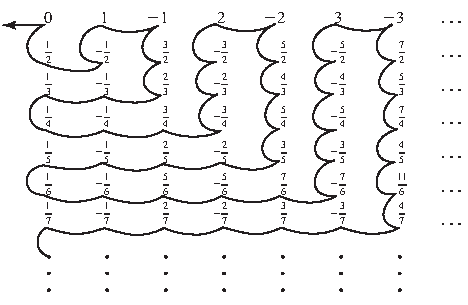
\includegraphics[width=0.642\linewidth,height=.8\textheight,keepaspectratio]{assets/p022_00.pdf}\end{center}
\begin{center}\small\textbf{0.15 Figure}\end{center}
\end{BookFloat}

\noindent downward, and contains all members of \BookInline{\mathbb{Q}.} We have shown a string winding its way through this array. Imagine the fractions to be glued to this string. Taking the beginning of the string and pulling to the left in the direction of the arrow, the string straightens out and all elements of \BookInline{\mathbb{Q}} appear on it in an infinite row as \BookInline{0,\allowbreak \frac{1}{2},\allowbreak - \frac{1}{2},\allowbreak 1,\allowbreak - 1,\allowbreak \frac{3}{2},\allowbreak \cdots.} Thus \BookInline{|\mathbb{Q}|= \aleph _{0}} also.

If the set \BookInline{S= \{x\in \mathbb{R}\mid 0<x<1\}} has cardinality \BookInline{\aleph _{0},\allowbreak } all its elements could be listed as unending decimals in a column extending infinitely downward, perhaps as

\[
\begin{array}{l}
0.3659663426\cdots\\
0.7103958453\cdots\\
0.0358493553\cdots\\
0.9968452214\cdots\\
\qquad\vdots
\end{array}
\]

\noindent We now argue that any such array must omit some number in \BookInline{S.} Surely \BookInline{S} contains a number \BookInline{r} having as its \BookInline{n}th digit after the decimal point a number different from 0, from 9, and from the \BookInline{n}th digit of the \BookInline{n}th number in this list. For example\BookInline{,\allowbreak r} might start \BookInline{.5637\cdots.} The 5 rather than 3 after the decimal point shows \BookInline{r} cannot be the first number in \BookInline{S} listed in the array shown. The 6 rather than 1 in the second digit shows \BookInline{r} cannot be the second number listed, and so on. Because we could make this argument with\textit{ any} \textit{list,} we see that \BookInline{S} has too many elements to be paired with those in \BookInline{\mathbb{Z}^{+ }.} Exercise 15 indicates that \BookInline{\mathbb{R}} has the same number of elements as \BookInline{S.} We just denote the cardinality of \BookInline{\mathbb{R}} by \BookInline{|\mathbb{R}|.} Exercise 19 indicates that there are infinitely many different cardinal numbers even greater than \BookInline{|\mathbb{R}|.}

\BookTextHeading{\textbf{Partitions and Equivalence Relations}  }

\noindent Sets are\textbf{ disjoint} if no two of them share a common element. In Example 0.17 we break up the integers into subsets. Eventually we will see how to define an algebraic structure on these subsets of \BookInline{\mathbb{Z}.} That is, we will be able to “add” two of these subsets to get another subset. We will find that breaking a set into subsets is a valuable tool in a number of settings, so we conclude this section with a brief study of\textit{ partitions} of sets.

\BookLabel{0.16 Definition} A\textbf{ partition} of a set \BookInline{S} is a collection of nonempty subsets of \BookInline{S} such that every element of \BookInline{S} is in exactly one of the subsets. The subsets are the\textbf{ cells} of the partition\BookInline{.}\BookEnd{\blacksquare}

\end{BookBody}

% Source PDF page 23; original printed page 6
\BookSource{23}{6}
\BookNarrativetrue

\begin{BookBody}

When discussing a partition of a set \BookInline{S,\allowbreak } we denote by \BookInline{\overline{x}} the cell containing the element \BookInline{x} of \BookInline{S.}

\BookLabel{0.17 Example} Splitting $\mathbb{Z}$ into the subset of even integers and the subset of odd integers, we obtain a partition of $\mathbb{Z}$ into the two cells listed below.
\[
\begin{aligned}
\overline{0}&=\{\ldots,-8,-6,-4,-2,0,2,4,\ldots\}\\
\overline{1}&=\{\ldots,-7,-5,-3,-1,1,3,5,\ldots\}
\end{aligned}
\]
We can think of $\overline{0}$ as being the integers that are divisible by $2$ and $\overline{1}$ as the integers that when divided by $2$ yield a remainder of $1$. This idea can be used for positive integers other than $2$. For example, we can partition $\mathbb{Z}$ into three cells:
\[
\begin{aligned}
\overline{0}&=\{x\in\mathbb{Z}\mid x\text{ is a multiple of }3\},\\
\overline{1}&=\{x\in\mathbb{Z}\mid\text{the remainder of }x\text{ divided by }3\text{ is }1\},\quad\text{and}\\
\overline{2}&=\{x\in\mathbb{Z}\mid\text{the remainder of }x\text{ divided by }3\text{ is }2\}.
\end{aligned}
\]
Note that when dividing a negative number by $3$, we still obtain a non-negative remainder. For example, $-5\div3$ is $-2$ with remainder $1$, which says that $\overline{-5}=\overline{1}$.

Generalizing, for each $n\in\mathbb{Z}^{+}$, we obtain a partition of $\mathbb{Z}$ consisting of $n$ cells, $\overline{0},\overline{1},\overline{2},\ldots,\overline{n-1}$. For each $0\leq r\leq n-1$, an integer $x$ is in the cell $\overline{r}$ exactly when the remainder of $x\div n$ is $r$. These cells are the \textbf{residue classes modulo} $n$ in $\mathbb{Z}$ and $n$ is called the \textbf{modulus}. We define the set $\mathbb{Z}/n\mathbb{Z}$ as the set containing the cells in this partition. So, for example, $\mathbb{Z}/3\mathbb{Z}=\{\overline{0},\overline{1},\overline{2}\}$. As we can see, $\mathbb{Z}/n\mathbb{Z}=\{\overline{0},\overline{1},\overline{2},\ldots,\overline{n-1}\}$ has exactly $n$ elements.\BookEnd{\blacktriangle}

Each partition of a set \BookInline{S} yields a relation \BookInline{\mathcal{R}} on \BookInline{S} in a natural way: namely, for \BookInline{x,\allowbreak y\in S,\allowbreak } let \BookInline{x\mathcal{R}y} if and only if \BookInline{x} and \BookInline{y} are in the same cell of the partition. In set notation, we would write \BookInline{x\mathcal{R}y} as \BookInline{(x,\allowbreak y)\in \mathcal{R}(}see Definition 0.7). A bit of thought shows that this relation \BookInline{\mathcal{R}} on \BookInline{S} satisfies the three properties of an\textit{ equivalence relation} in the following definition.

\BookLabel{0.18 Definition} An\textbf{ equivalence relation} \BookInline{\mathcal{R}} on a set \BookInline{S} is one that satisfies these three properties for all \BookInline{x,\allowbreak y,\allowbreak z\in S.}

\BookExercise{1.}{(Reflexive\BookInline{)\; x\mathcal{R}x.}}

\BookExercise{2.}{(Symmetric) If \BookInline{x\mathcal{R}y,\allowbreak } then \BookInline{y\mathcal{R}x.}}

\BookExercise{3.}{(Transitive) If \BookInline{x\mathcal{R}y} and \BookInline{y\mathcal{R}z} then \BookInline{x\mathcal{R}z.}} \BookEnd{\blacksquare}

To illustrate why the relation \BookInline{\mathcal{R}} corresponding to a partition of \BookInline{S} satisfies the symmetric condition in the definition, we need only observe that if \BookInline{y} is in the same cell as \BookInline{x} (that is, if \BookInline{x\mathcal{R}y),\allowbreak } then \BookInline{x} is in the same cell as \BookInline{y(}that is\BookInline{,\allowbreak y\mathcal{R}x).} We leave the similar observations to verify the reflexive and transitive properties to Exercise 28.

\BookLabel{0.19 Example} For any nonempty set \BookInline{S,\allowbreak } the equality relation \BookInline{= } defined by the subset \BookInline{\{(x,\allowbreak x)\mid x\in S\}} of \BookInline{S\times S} is an equivalence relation\BookInline{.}\BookEnd{\blacktriangle}

\BookLabel{0.20 Example} \textbf{(Congruence Modulo} \BookInline{n)} Let \BookInline{n\in \mathbb{Z}^{+ }.} The equivalence relation on \BookInline{\mathbb{Z}} corresponding to the partition of \BookInline{\mathbb{Z}} into residue classes modulo \BookInline{n,\allowbreak } discussed in Example 0.17, is\textbf{ con}\textbf{gruence modulo} \BookInline{n.} It is sometimes denoted by \BookInline{\equiv _{n}.} Rather than write \BookInline{a\equiv _{n}b,\allowbreak } we usually write \BookInline{a\equiv b(}mod \BookInline{n),\allowbreak } read, “\BookInline{a} is congruent to \BookInline{b} modulo \BookInline{n.}” For example, we have \BookInline{15\equiv 27(}mod 4) because both 15 and 27 have remainder 3 when divided by \BookInline{4.}\BookEnd{\blacktriangle}

\end{BookBody}

% Source PDF page 24; original printed page 7
\BookSource{24}{7}
\BookNarrativetrue

\begin{BookBody}

\BookLabel{0.21 Example} Let a relation \BookInline{\mathcal{R}} on the set \BookInline{\mathbb{Z}} be defined by \BookInline{n\mathcal{R}m} if and only if \BookInline{nm\geq 0,\allowbreak } and let us determine whether \BookInline{\mathcal{R}} is an equivalence relation.

\textbf{Reflexive} \BookInline{a\mathcal{R}a,\allowbreak } because \BookInline{a^{2}\geq 0} for all \BookInline{a\in \mathbb{Z}.}

\textbf{Symmetric} If \BookInline{a\mathcal{R}b,\allowbreak } then \BookInline{ab\geq 0,\allowbreak } so \BookInline{ba\geq 0} and \BookInline{b\mathcal{R}a.}

\textbf{Transitive} If \BookInline{a\mathcal{R}b} and \BookInline{b\mathcal{R}c,\allowbreak } then \BookInline{ab\geq 0} and \BookInline{bc\geq 0.} Thus \BookInline{ab^{2}c= acb^{2}\geq 0.}

If we knew \BookInline{b^{2}>0,\allowbreak } we could deduce\textit{ ac} \BookInline{\geq 0} whence \BookInline{a\mathcal{R}c.} We have to examine the case \BookInline{b= 0} separately. A moment of thought shows that \BookInline{- 3\mathcal{R}0} and \BookInline{0\mathcal{R}5,\allowbreak } but we do\textit{ not} have \BookInline{- 3\mathcal{R}5.} Thus the relation \BookInline{\mathcal{R}} is not transitive, and hence is not an equivalence relation\BookInline{.}\BookEnd{\blacktriangle}

We observed above that a partition yields a natural equivalence relation. We now show that an equivalence relation on a set yields a natural partition of the set. The theorem that follows states both results for reference.

\BookLabel{0.22 Theorem} \textbf{(Equivalence Relations and Partitions)} Let \BookInline{S} be a nonempty set and let \BookInline{\sim } be an equivalence relation on \BookInline{S.} Then \BookInline{\sim } yields a partition of \BookInline{S,\allowbreak } where

\begin{center}\begin{adjustbox}{max width=\linewidth}\BookInline{\displaystyle \overline{a}= \{x\in S\mid x\sim a\}.}\end{adjustbox}\end{center}

\noindent Also, each partition of \BookInline{S} gives rise to an equivalence relation \BookInline{\sim } on \BookInline{S} where \BookInline{a\sim b} if and only if \BookInline{a} and \BookInline{b} are in the same cell of the partition.

\BookLabel{\textit{Proof}} We must show that the different cells $\overline{a}=\{x\in S\mid x\sim a\}$ for $a\in S$ do give a partition of $S$, so that every element of $S$ is in some cell and so that if $a\in\overline{b}$, then $\overline{a}=\overline{b}$. Let $a\in S$. Then $a\in\overline{a}$ by the reflexive condition (1), so $a$ is in \textit{at least one} cell.

Suppose now that $a\in\overline{b}$. We need to show that $\overline{a}=\overline{b}$ as sets; this will show that $a$ cannot be in more than one cell. There is a standard way to show that two sets are the same:
\begin{center}\textit{Show that each set is a subset of the other.}\end{center}
\noindent We show that $\overline{a}\subseteq\overline{b}$. Let $x\in\overline{a}$. Then $x\sim a$. But $a\in\overline{b}$, so $a\sim b$. Then, by the transitive condition (3), $x\sim b$, so $x\in\overline{b}$. Thus $\overline{a}\subseteq\overline{b}$. Now we show that $\overline{b}\subseteq\overline{a}$. Let $y\in\overline{b}$. Then $y\sim b$. But $a\in\overline{b}$, so $a\sim b$ and, by symmetry (2), $b\sim a$. Then by transitivity (3), $y\sim a$, so $y\in\overline{a}$. Hence $\overline{b}\subseteq\overline{a}$ also, so $\overline{b}=\overline{a}$ and our proof is complete.\BookEnd{\blacklozenge}

Each cell in the partition arising from an equivalence relation is an\textbf{ equivalence} \textbf{class}.

\end{BookBody}

\BookNarrativefalse

\begin{BookBody}

\BookExerciseTitle{0}

\noindent In Exercises 1 through 4, describe the set by listing its elements.

\BookExercise{1.}{\BookInline{\{x\in \mathbb{R}\mid x^{2}= 3\}}}

\BookExercise{2.}{$\{m\in\mathbb{Z}\mid m^2+m=6\}$}

\BookExercise{3.}{\BookInline{\{m\in \mathbb{Z}\mid mn= 60} for some \BookInline{n\in \mathbb{Z}\}}}

\BookExercise{4.}{\BookInline{\{x\in \mathbb{Z}\mid x^{2}- 10x+ 16\leq 0\}}}

\noindent In Exercises 5 through 10, decide whether the object described is indeed a set (is well defined). Give an alternate description of each set.

\BookExercise{5.}{\BookInline{\{n\in \mathbb{Z}^{+ }\mid n} is a large number\BookInline{\}}}

\BookExercise{6.}{\BookInline{\{n\in \mathbb{Z}\mid n^{2}<0\}}}

\BookExercise{7.}{\BookInline{\{n\in \mathbb{Z}\mid 39<n^{3}<57\}}}

\BookExercise{8.}{\BookInline{\{r\in \mathbb{Q}\mid } When \BookInline{r} is multiplied by a sufficiently large power of 2, one obtains a whole number\BookInline{.\}}}

\BookExercise{9.}{\BookInline{\{x\in \mathbb{Z}^{+ }\mid x} is an easy number to factor\BookInline{\}}}

\BookExercise{10.}{\BookInline{\{x\in \mathbb{Q}\mid x} may be written with positive denominator less than \BookInline{4\}}}

\BookExercise{11.}{List the elements in \BookInline{\{a,\allowbreak b,\allowbreak c\}\times \{1,\allowbreak 2,\allowbreak c\}.}}

\end{BookBody}

% Source PDF page 25; original printed page 8
\BookSource{25}{8}
\BookNarrativefalse

\begin{BookBody}

\begin{BookFloat}{00_sets_and_relations-p25-0}
\begin{center}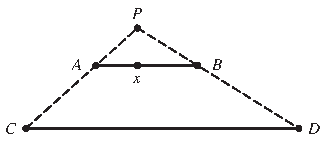
\includegraphics[width=0.445\linewidth,height=.8\textheight,keepaspectratio]{assets/p025_00.pdf}\end{center}
\begin{center}\small\textbf{0.23 Figure}\end{center}
\end{BookFloat}

\BookExercise{12.}{Let \BookInline{A= \{1,\allowbreak 2,\allowbreak 3\}} and \BookInline{B= \{2,\allowbreak 4,\allowbreak 6\}.} For each relation between \BookInline{A} and \BookInline{B} given as a subset of \BookInline{A\times B,\allowbreak } decide whether it is a function mapping \BookInline{A} into \BookInline{B.} If it is a function, decide whether it is one-to-one and whether it is onto \BookInline{B.} \textbf{a}\BookInline{.\{\{1,\allowbreak 2\},\allowbreak \{2,\allowbreak 6\},\allowbreak \{3,\allowbreak 4\}\}} \textbf{b.} [[1,3] and [5,7]] \textbf{c}\BookInline{.\{(1,\allowbreak 6),\allowbreak (1,\allowbreak 2),\allowbreak (1,\allowbreak 4)\}} \textbf{d}\BookInline{.\{\{2,\allowbreak 2\},\allowbreak \{3,\allowbreak 6\},\allowbreak \{1,\allowbreak 6\}\}} \textbf{e}\BookInline{.\{(1,\allowbreak 6),\allowbreak (2,\allowbreak 6),\allowbreak (3,\allowbreak 6)\}} \textbf{f}\BookInline{.\{\{1,\allowbreak 2\},\allowbreak \{2,\allowbreak 6\}\}}}

\BookExercise{13.}{Illustrate geometrically that two line segments \BookInline{AB} and \BookInline{CD} of different lengths have the same number of points by indicating in Fig. 0.23 what point \BookInline{y} of \BookInline{CD} might be paired with point \BookInline{x} of \BookInline{AB.}}

\BookExercise{14.}{Recall that for \BookInline{a,\allowbreak b\in \mathbb{R}} and \BookInline{a<b,\allowbreak } the\textbf{ closed interval} \BookInline{[a,\allowbreak b]} in \BookInline{\mathbb{R}} is defined by \BookInline{[a,\allowbreak b]= \{x\in \mathbb{R}\mid a\leq x\leq } \BookInline{b\}.} Show that the given intervals have the same cardinality by giving a formula for a one-to-one function \BookInline{f} mapping the first interval onto the second. \textbf{a.} [0, 1] and [0, 2] \textbf{b.} [1, 3] and [5, 7] \textbf{c}\BookInline{.[a,\allowbreak b]} and \BookInline{[c,\allowbreak d]}}

\BookExercise{15.}{Show that \BookInline{S= \{x\in \mathbb{R}\mid 0<x<1\}} has the same cardinality as \BookInline{\mathbb{R}.[}\textit{Hint:} Find an elementary function of calculus that maps an interval one-to-one onto \BookInline{\mathbb{R},\allowbreak } and then translate and scale appropriately to make the domain the set \BookInline{S.]}}

\noindent For any set \BookInline{A,\allowbreak } we denote by \BookInline{\mathcal{P}(A)} the collection of all subsets of \BookInline{A.} For example, if \BookInline{A= \{a,\allowbreak b,\allowbreak c,\allowbreak d\},\allowbreak } then \BookInline{\{a,\allowbreak b,\allowbreak d\}\in } \BookInline{\mathcal{P}(A).} The set \BookInline{\mathcal{P}(A)} is the\textbf{ power set} of \BookInline{A.} Exercises 16 through 19 deal with the notion of the power set of a set \BookInline{A.}

\BookExercise{16.}{List the elements of the power set of the given set and give the cardinality of the power set. \textbf{a}\BookInline{.\emptyset } \textbf{b}\BookInline{.\{a\}} \textbf{c}\BookInline{.\{a,\allowbreak b\}} \textbf{d}\BookInline{.\{a,\allowbreak b,\allowbreak c\}}}

\BookExercise{17.}{Let \BookInline{A} be a finite set, and let \BookInline{|A|= s.} Based on the preceding exercise, make a conjecture about the value of \BookInline{|\mathcal{P}(A)|.} Then try to prove your conjecture.}

\BookExercise{18.}{For any set \BookInline{A,\allowbreak } finite or infinite, let \BookInline{B^{A}} be the set of all functions mapping \BookInline{A} into the set \BookInline{B= \{0,\allowbreak 1\}.} Show that the cardinality of \BookInline{B^{A}} is the same as the cardinality of the set \BookInline{\mathcal{P}(A).[}\textit{Hint:} Each element of \BookInline{B^{A}} determines a subset of \BookInline{A} in a natural way.]}

\BookExercise{19.}{Show that the power set of a set \BookInline{A,\allowbreak } finite or infinite, has too many elements to be able to be put in a one-to-one correspondence with \BookInline{A.} Explain why this intuitively means that there are an infinite number of infinite cardinal numbers. [\textit{Hint:} Imagine a one-to-one function \BookInline{\phi } mapping \BookInline{A} into \BookInline{\mathcal{P}(A)} to be given. Show that \BookInline{\phi } cannot be onto \BookInline{\mathcal{P}(A)} by considering, for each \BookInline{x\in A,\allowbreak } whether \BookInline{x\in \phi (x)} and using this idea to define a subset \BookInline{S} of \BookInline{A} that is not in the range of \BookInline{\phi.]} Is\textit{ the set of everything} a logically acceptable concept? Why or why not?}

\BookExercise{20.}{Let \BookInline{A= \{1,\allowbreak 2\}} and let \BookInline{B= \{3,\allowbreak 4,\allowbreak 5\}.}}

\BookExercise{a.}{Illustrate, using \BookInline{A} and \BookInline{B,\allowbreak } why we consider that \BookInline{2+ 3= 5.} Use similar reasoning with sets of your own choice to decide what you would consider to be the value of}

\noindent
\begin{tabular*}{\linewidth}{@{\extracolsep{\fill}}ll@{}}
\textnormal{i.}\quad $3+\aleph_0,$ & \textnormal{ii.}\quad $\aleph_0+\aleph_0.$
\end{tabular*}

\BookExercise{b.}{Illustrate why we consider that \BookInline{2\cdot 3= 6} by plotting the points of \BookInline{A\times B} in the plane \BookInline{\mathbb{R}\times \mathbb{R}.} Use similar reasoning with a figure in the text to decide what you would consider to be the value of \BookInline{\aleph _{0}\cdot \aleph _{0}.}}

\BookExercise{21.}{How many numbers in the interval \BookInline{0\leq x\leq 1} can be expressed in the form.\#\#, where each \# is a digit \BookInline{0,\allowbreak 1,\allowbreak 2,\allowbreak 3,\allowbreak \cdots,\allowbreak 9}? How many are there of the form.\#\#\#\#\#? Following this idea, and Exercise 15, decide what you would consider to be the value of \BookInline{10^{\aleph _{0}}.} How about \BookInline{12^{\aleph _{0}}} and \BookInline{2^{\aleph _{0}}}?}

\end{BookBody}

% Source PDF page 26; original printed page 9
\BookSource{26}{9}
\BookNarrativefalse

\begin{BookBody}

\BookExercise{22.}{Continuing the idea in the preceding exercise and using Exercises 18 and 19, use exponential notation to fill in the three blanks to give a list of five cardinal numbers, each of which is greater than the preceding one.}

\BookInline{\aleph _{0},\allowbreak |\mathbb{R}|,\allowbreak _{- - - },\allowbreak _{- - - },\allowbreak _{- - - }.}

\noindent In Exercises 23 through 27, find the number of different partitions of a set having the given number of elements.

\BookExercise{23.}{1 element}

\BookExercise{24.}{2 elements}

\BookExercise{25.}{3 elements}

\BookExercise{26.}{4 elements}

\BookExercise{27.}{5 elements}

\BookExercise{28.}{Consider a partition of a set $S$. The paragraph following Definition 0.18 explained why the relation $x\mathcal{R}y$ if and only if $x$ and $y$ are in the same cell satisfies the symmetric condition for an equivalence relation. Write similar explanations of why the reflexive and transitive properties are also satisifed.}

\noindent In Exercises 29 through 34, determine whether the given relation is an equivalence relation on the set. Describe the partition arising from each equivalence relation.

\BookExercise{29.}{\BookInline{n\mathcal{R}m} in \BookInline{\mathbb{Z}} if \BookInline{nm>0}}

\BookExercise{30.}{\BookInline{x\mathcal{R}y} in \BookInline{\mathbb{R}} if \BookInline{x\geq y}}

\BookExercise{31.}{\BookInline{x\mathcal{R}y} in \BookInline{\mathbb{Z}^{+ }} if the greatest common divisor of \BookInline{x} and \BookInline{y} is greater than 1}

\BookExercise{32.}{\BookInline{(x_{1},\allowbreak y_{1})\mathcal{R}(x_{2},\allowbreak y_{2})} in \BookInline{\mathbb{R}\times \mathbb{R}} if \BookInline{x_{1}^{2}+ y_{1}^{2}= x_{2}^{2}+ y_{2}^{2}}}

\BookExercise{33.}{\BookInline{n\mathcal{R}m} in \BookInline{\mathbb{Z}^{+ }} if \BookInline{n} and \BookInline{m} have the same number of digits in the usual base ten notation}

\BookExercise{34.}{\BookInline{n\mathcal{R}m} in \BookInline{\mathbb{Z}^{+ }} if \BookInline{n} and \BookInline{m} have the same final digit in the usual base ten notation}

\BookExercise{35.}{Using set notation of the form \BookInline{\{...,\allowbreak } \#, \#, \#\BookInline{,\allowbreak \cdots \},\allowbreak } write the residue classes modulo \BookInline{n} in \BookInline{\mathbb{Z}} as discussed in Example 0.17 for the indicated values of \BookInline{n.} \textbf{a.} 3 \textbf{b.} 4 \textbf{c.} 5}

\BookExercise{36.}{Write each set by listing its elements. \textbf{b}\BookInline{.\mathbb{Z}/4\mathbb{Z}} \textbf{c}\BookInline{.\mathbb{Z}/5\mathbb{Z}} \textbf{a}\BookInline{.\mathbb{Z}/3\mathbb{Z}}}

\BookExercise{37.}{When discussing residue classes, 1 is not well defined until the modulus \BookInline{n} is given. Explain.}

\BookExercise{38.}{Let \BookInline{n\in \mathbb{Z}^{+ }} and let \BookInline{\sim } be defined on \BookInline{\mathbb{Z}} by \BookInline{r\sim s} if and only if \BookInline{r- s} is divisible by \BookInline{n,\allowbreak } that is, if and only if \BookInline{r- s= nq} for some \BookInline{q\in \mathbb{Z}.}}

\BookExercise{a.}{Show that \BookInline{\sim } is an equivalence relation on \BookInline{\mathbb{Z}.}}

\BookExercise{b.}{Show that this \BookInline{\sim } is the equivalence relation,\textit{ congruence modulo} \BookInline{n,\allowbreak } of Example 0.20.}

\BookExercise{39.}{Let \BookInline{n\in \mathbb{Z}^{+ }.} Using the relation from Exercise 38, show that if \BookInline{a_{1}\sim a_{2}} and \BookInline{b_{1}\sim b_{2},\allowbreak } then \BookInline{(a_{1}+ b_{1})} \BookInline{\sim (a_{2}+ b_{2}).}}

\BookExercise{40.}{Let \BookInline{n\in \mathbb{Z}^{+ }.} Using the relation from Exercise 38, show that if \BookInline{a_{1}\sim a_{2}} and \BookInline{b_{1}\sim b_{2},\allowbreak } then \BookInline{(a_{1}b_{1})\sim (a_{2}b_{2}).}}

\BookExercise{41.}{Students often misunderstand the concept of a one-to-one function (mapping). I think I know the reason. You see, a mapping \BookInline{\phi:A\to B} has a\textit{ direction} associated with it, from \BookInline{A} to \BookInline{B.} It seems reasonable to expect a one-to-one mapping simply to be a mapping that carries one point of \BookInline{A} into one point of \BookInline{B,\allowbreak } in the direction indicated by the arrow. But of course,\textit{ every} mapping of \BookInline{A} into \BookInline{B} does this, and Definition 0.12 did not say that at all. With this unfortunate situation in mind, make as good a pedagogical case as you can for calling the functions described in Definition 0.12\textit{ two-to-two functions} instead. (Unfortunately, it is almost impossible to get widely used terminology changed.)}

\end{BookBody}
\ifdefined\BookMaster\let\BookFinish\relax\else\def\BookFinish{\end{document}}\fi\BookFinish
